%\title{Project Report}
%
%%% Preamble
\documentclass[paper=a4, fontsize=11pt]{scrartcl}
\usepackage[T1]{fontenc}
\usepackage{fourier}
\usepackage{listings}

\usepackage[english]{babel}															% English language/hyphenation
\usepackage[protrusion=true,expansion=true]{microtype}	
\usepackage{amsmath,amsfonts,amsthm} % Math packages
\usepackage[pdftex]{graphicx}	
\usepackage{url}
\usepackage{hyperref}
\usepackage{graphicx}
\usepackage{wrapfig}
\usepackage[margin=1.00in]{geometry}
\usepackage{amsmath}
\usepackage[]{algorithm2e}

%%% Custom sectioning
\usepackage{sectsty}
\allsectionsfont{\centering \normalfont\scshape}


%%% Custom headers/footers (fancyhdr package)
\usepackage{fancyhdr}
\pagestyle{fancyplain}
\fancyhead{}											% No page header
\fancyfoot[L]{}											% Empty 
\fancyfoot[C]{}											% Empty
\fancyfoot[R]{\thepage}									% Pagenumbering
\renewcommand{\headrulewidth}{0pt}			% Remove header underlines
\renewcommand{\footrulewidth}{0pt}				% Remove footer underlines
\setlength{\headheight}{3.6pt}
\date{}


%%% Equation and float numbering
\numberwithin{equation}{section}		% Equationnumbering: section.eq#
\numberwithin{figure}{section}			% Figurenumbering: section.fig#
\numberwithin{table}{section}				% Tablenumbering: section.tab#


%%% Maketitle metadata
\newcommand{\horrule}[1]{\rule{\linewidth}{#1}} 	% Horizontal rule

\title{
		\vspace{-1in} 	
		\usefont{OT1}{bch}{b}{n}
		\normalfont \normalsize \textsc{Durham Computer Science} \\ [5pt]
		\horrule{0.5pt} \\[0.4cm]
		\huge  Network Analysis Assignment - LLLL76\\
		\horrule{2pt} \\[0.5cm]
		\vspace{-1in} 	
}

%%% Begin document
\begin{document}
\maketitle
%%%%%%%%%%%%%%%%%%%%%%%%%%%%%%%%%%%%%%%%%%%%%%%%%%
\section*{Question One}

A Group Graph is defined by four parameters m, k, p and q and is constructed as follows:
\begin{itemize}
  \item Create m*k vertices. The vertices are partitioned into m groups each of size k.
  \item For each pair of vertices that belong to the same group, add an edge between them with
probability p.
  \item For each pair of vertices that belong to different groups, add an edge between them
with probability q.
\end{itemize}
	
We will choose arbitrary m and k to test the structure change of p and q, we choose values of p and q such that p + q = 0.5, p > q. The values of m and k will then be changed so as to cover three different test criteria over all values of p and q, they are then compared to the baseline. The three test criteria for values of m and k are such that m < k, m = k, and m > k.\\

In theory at higher values of p and lower values of q the structure of the graph will be groups of nodes that are highly interconnected with significantly fewer connections between these groups, at lower values of p and higher values of q as p and q come together we get closer to seeing a random graph with the probability of an edge being present inside a group and between two groups being similar, if the probability was exactly the same then we would see a random graph with a set probability of any two nodes being connected irrespective of what group they are in. The values of m and k are unlikely to change all that much with regards to the connections that we see as part of the structure to the graph. If we take the two extremes of our testing range, high p, low q and then lower p, higher q, in the instance of a high p, low q for m > k we will see a high number of small highly interconnected groups with few 'between group'  edges. For the same values of m and k but with a lower p and higher q value we will see a structure that closely resembles a random graph with slightly more interconnects inside each group. In the final case of m < k for the two extremes of our p and q values, at high p and low q we would expect to see large highly connected groups with little in the way of inter group edges. Then for lower p and higher q we see the same trend towards a random graph but still with the same higher number of edges intra group as p != q.\\

In the first round of testing we want m and k to be equal, m = 20, k = 20, p = [0.45, 0.4, 0.35, 0.3], and q = [0.05, 0.1, 0.15, 0.2]. The degree distribution is shown in figure 0.1.

\begin{figure}[h]
\center
\caption{M = 20, K = 20, with [P,Q] varying: [0.3,0.2], [0.35,0.15], [0.4,0.1], [0.45,0.05] respectively.}
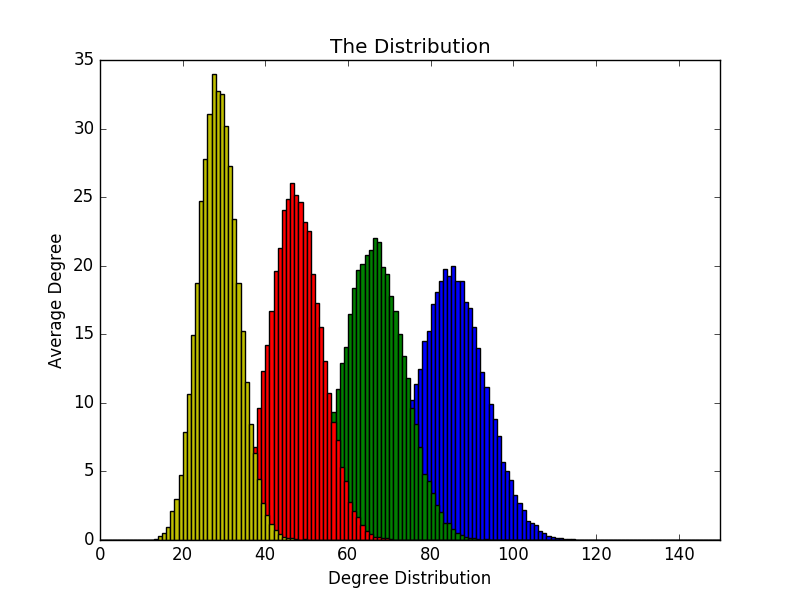
\includegraphics[width=0.75\textwidth]{pictures/m=k.png}
\end{figure}

\begin{figure}[h]
\center
\caption{M = 5, K = 5, with [P,Q] varying: [0.3,0.2], [0.35,0.15], [0.4,0.1], [0.45,0.05] respectively.}
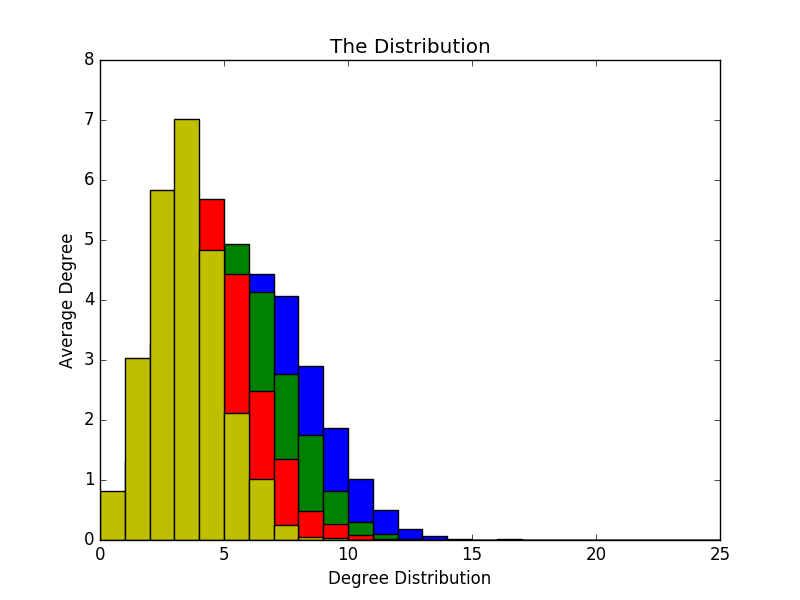
\includegraphics[width=0.75\textwidth]{pictures/k=m.png}
\end{figure}

Second round of testing, m > k, m = 20, k = 5, p = [0.45, 0.4, 0.35, 0.3], and q = [0.05, 0.1, 0.15, 0.2]. The degree distribution is shown in figure 0.2.

\begin{figure}[h]
\center
\caption{M = 5, K = 20, with [P,Q] varying: [0.3,0.2], [0.35,0.15], [0.4,0.1], [0.45,0.05] respectively.}
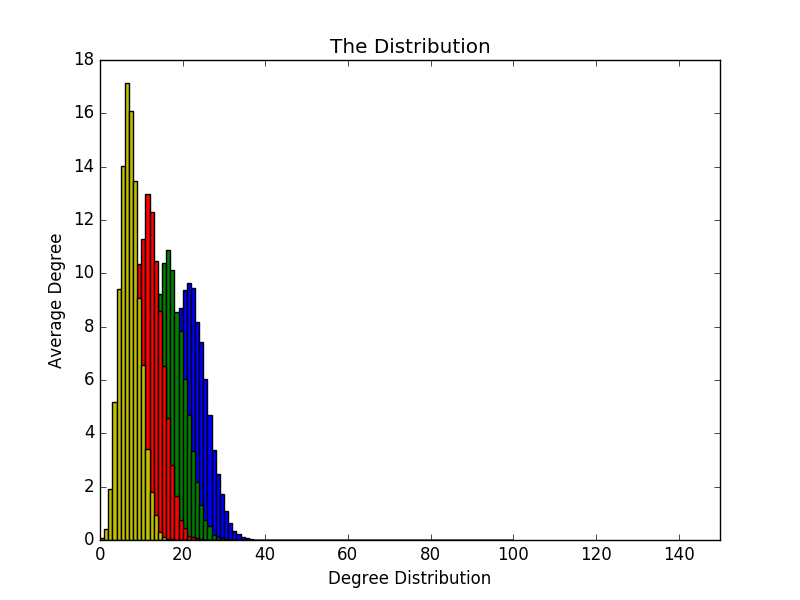
\includegraphics[width=0.75\textwidth]{pictures/m>k.png}
\end{figure}

Third round of testing, m < k, m = 5, k = 20, p = [0.45, 0.4, 0.35, 0.3], and q = [0.05, 0.1, 0.15, 0.2]. The degree distribution is shown in figure 0.3.

\begin{figure}[h]
\center
\caption{M = 20, K = 5, with [P,Q] varying: [0.3,0.2], [0.35,0.15], [0.4,0.1], [0.45,0.05] respectively.}
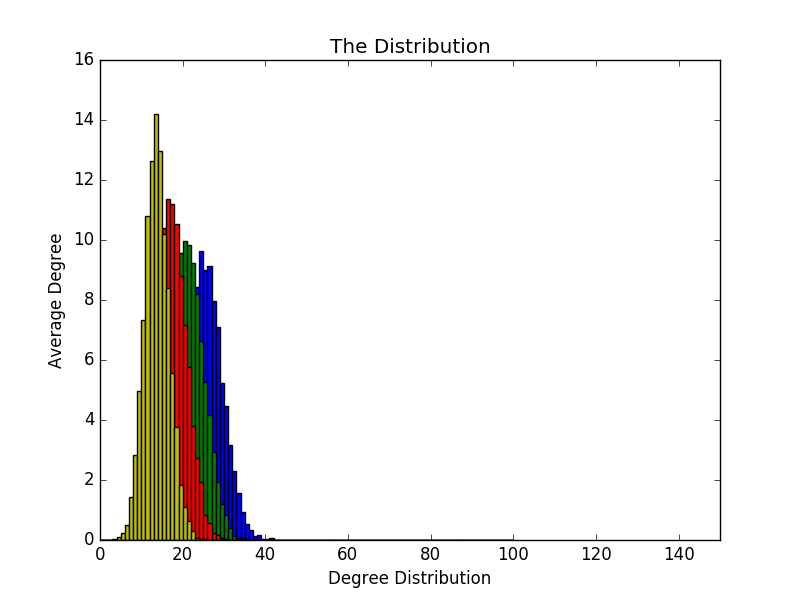
\includegraphics[width=0.75\textwidth]{pictures/m<k.png}
\end{figure}

\subsection*{Diameter}

Using the values m = 50, k = 5, q = 0.1, run an average diameter over 100 graphs with variable p values gives the graph figure 0.5.

\begin{figure}[h]
\center
\caption{}
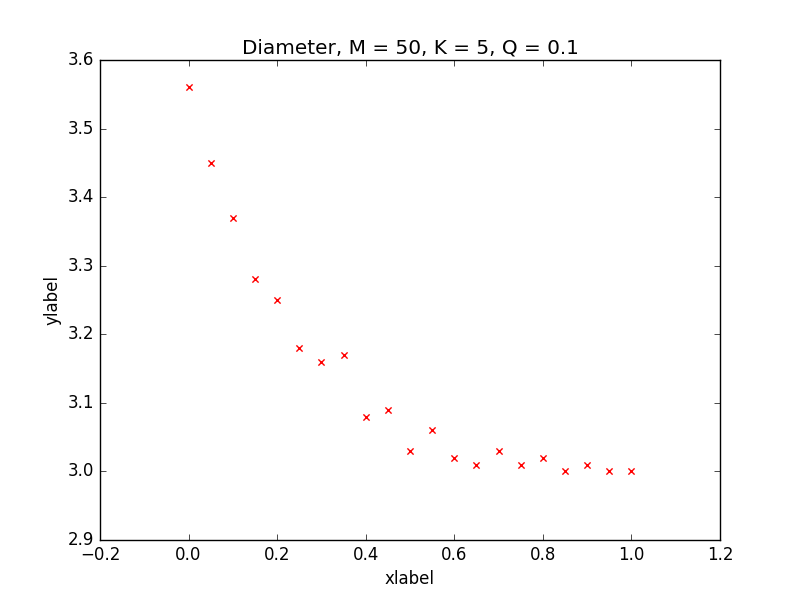
\includegraphics[width=0.75\textwidth]{pictures/diameter.png}
\end{figure}

As the graph shows the average over all values of p is around 3 and it will converge to 3 for higher values of p. At higher P values there is a higher probability that there is an intra-group connection, whilst the Q value is fixed, meaning that there is a set probability of an inter-group connection. With higher values of probability for intra-group connections this will reduce the possible diameter due to the fact that if each group was strongly connected then the average path between any pair of nodes would be two that were in separate groups but unconnected, thus the travel to any node in the start group that is connected to any node in the target group which would then be connected to the target node, there will be a few exceptions such as two nodes in two groups that have no nodes connected, this is why the average for p = 1 is slightly above 3. Whilst we can see an obvious trend in the graph, due to the parameters chosen this is highly magnified, with most other values that were tested we see a much flatter result, shown in figure 0.6.

\begin{figure}[h]
\center
\caption{}
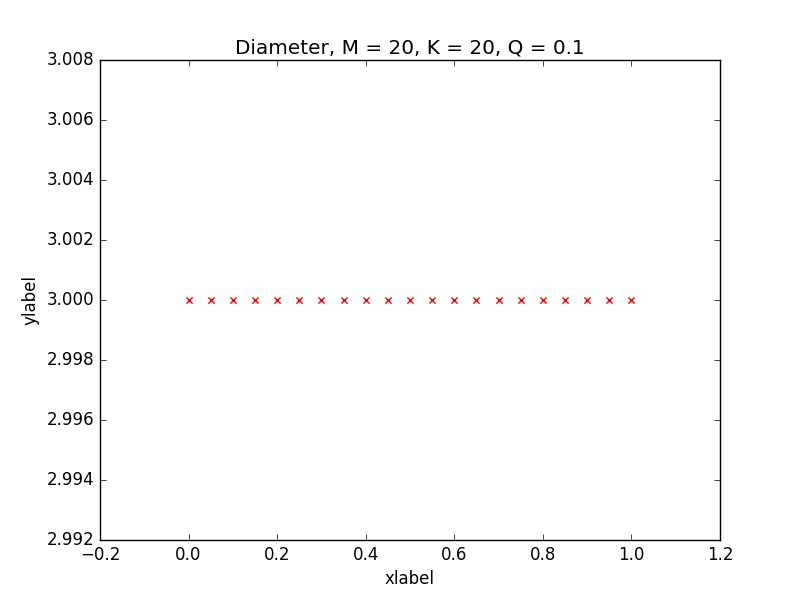
\includegraphics[width=0.75\textwidth]{pictures/otherD.png}
\end{figure}

%%%%%%%%%%%%%%%%%%%%%%%%%%%%%%%%%%%%%%%%%%%%%%%%%%
\section*{Question Two}

A k-cycle is a set of k vertices {1, 2, . . . , k} such that 1 is joined to 2, 2 is joined to 3, . . .,
and k is joined to 1 (it does not matter whether or not other vertices are adjacent). For k = 4 and k = 5, find out for a random sample of the vertices, how many k-cycles each vertex belongs to and plot the distribution for the co-authorship, random, PA, and group graphs. All graphs are undirected.

\subsection*{Four Cycles}

\begin{figure}[h]
\center
\caption{}
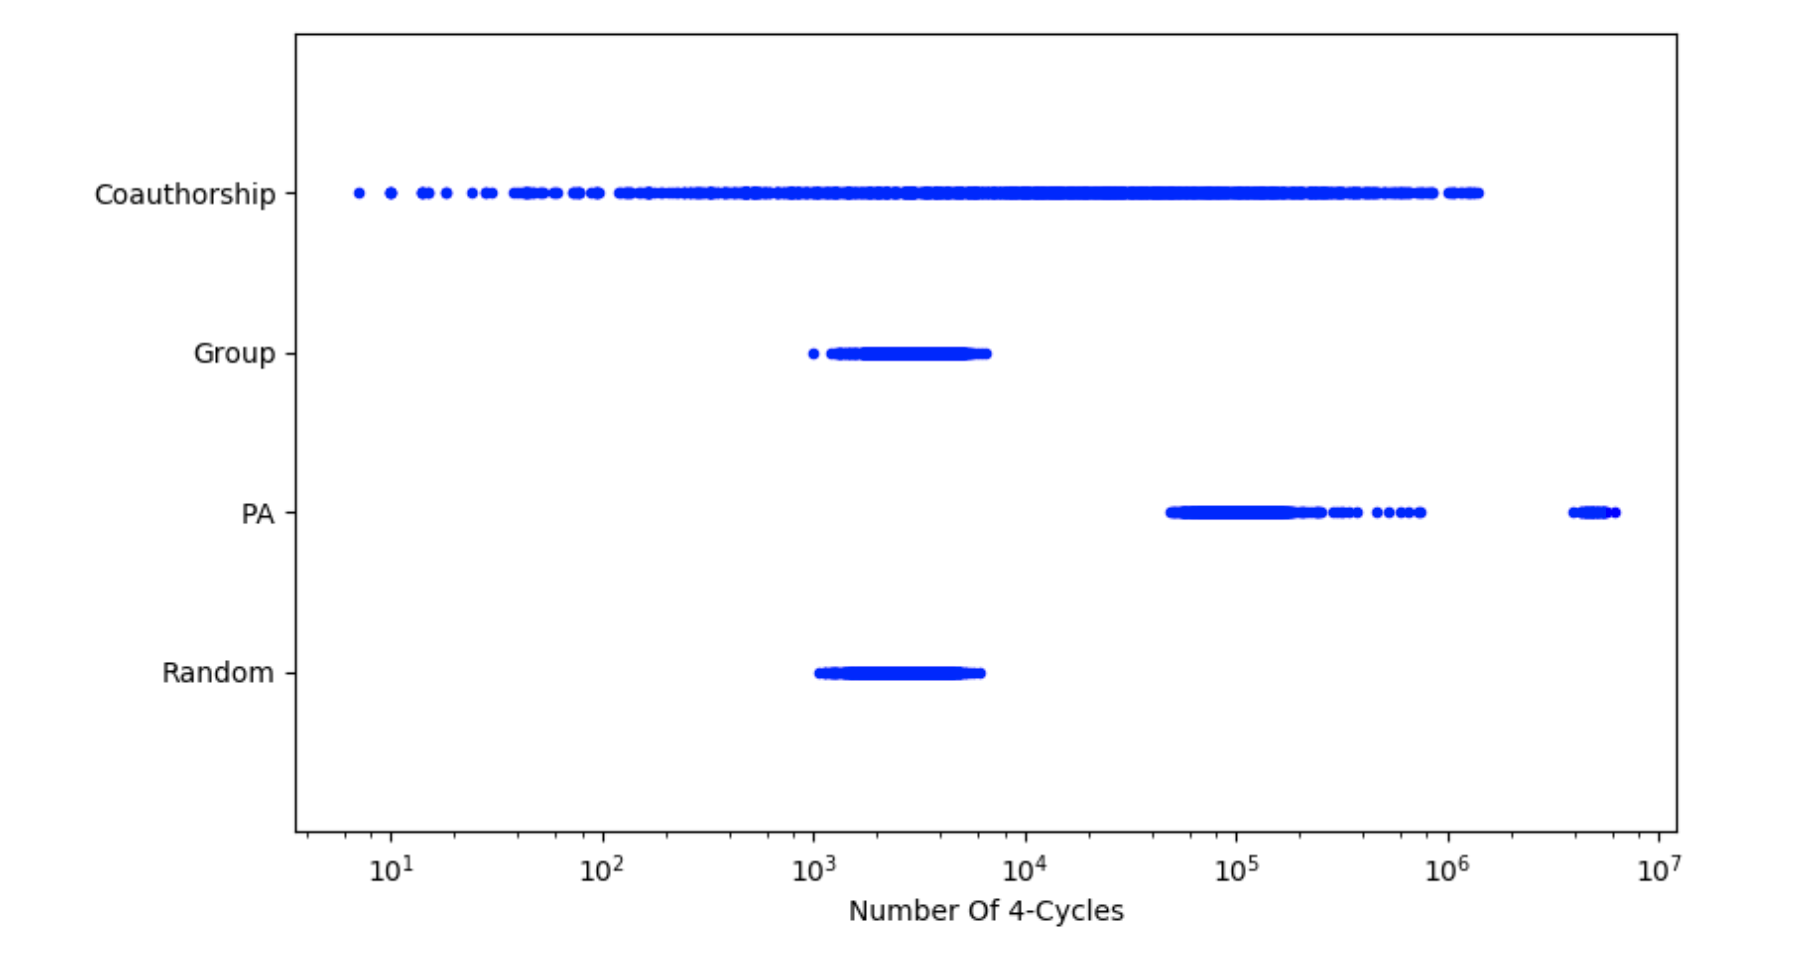
\includegraphics[width=0.75\textwidth]{pictures/4cycle.png}
\end{figure}

As shown in figure 0.7 the co-authorship graph any given node could be in a significant range of 4-cycles, from 10 to 1000000. As shown from the graph none of the other graphs make an accurate model of the co-authorship graph. \\
The group graph, with parameters m = 40, k = 40, p = 0.5, and q = 0.02, shows a fairly condensed range of values, this would be due to the limited amount of inter-group connections that occur through a low q value. This would result in limiting the spread as there would be very few cycles that would be inter-group resulting in a cap being present in the number that can occur within a group.\\
The PA graph, with parameters nodes = 1600 and out degree = 35, shows two separate groups, with the higher being much smaller, this could be due to the much smaller collection of fully connected nodes that make up the core of the PA graph. The fully connected sub-graph would be present in many more 4-cycles than any of the other nodes that are added after this code group is created. This is due to the nature of a fully connected graph. \\
Finally the random graph, parameters nodes = 1600 and probability = 0.02, shows a fairly small range of possible values, and is very similar to the group graph is size and range. This could be due to the similarity that the q value of the group graph and the probability of the random graph share. 

\subsection*{Five Cycles}

\begin{figure}[h]
\center
\caption{}
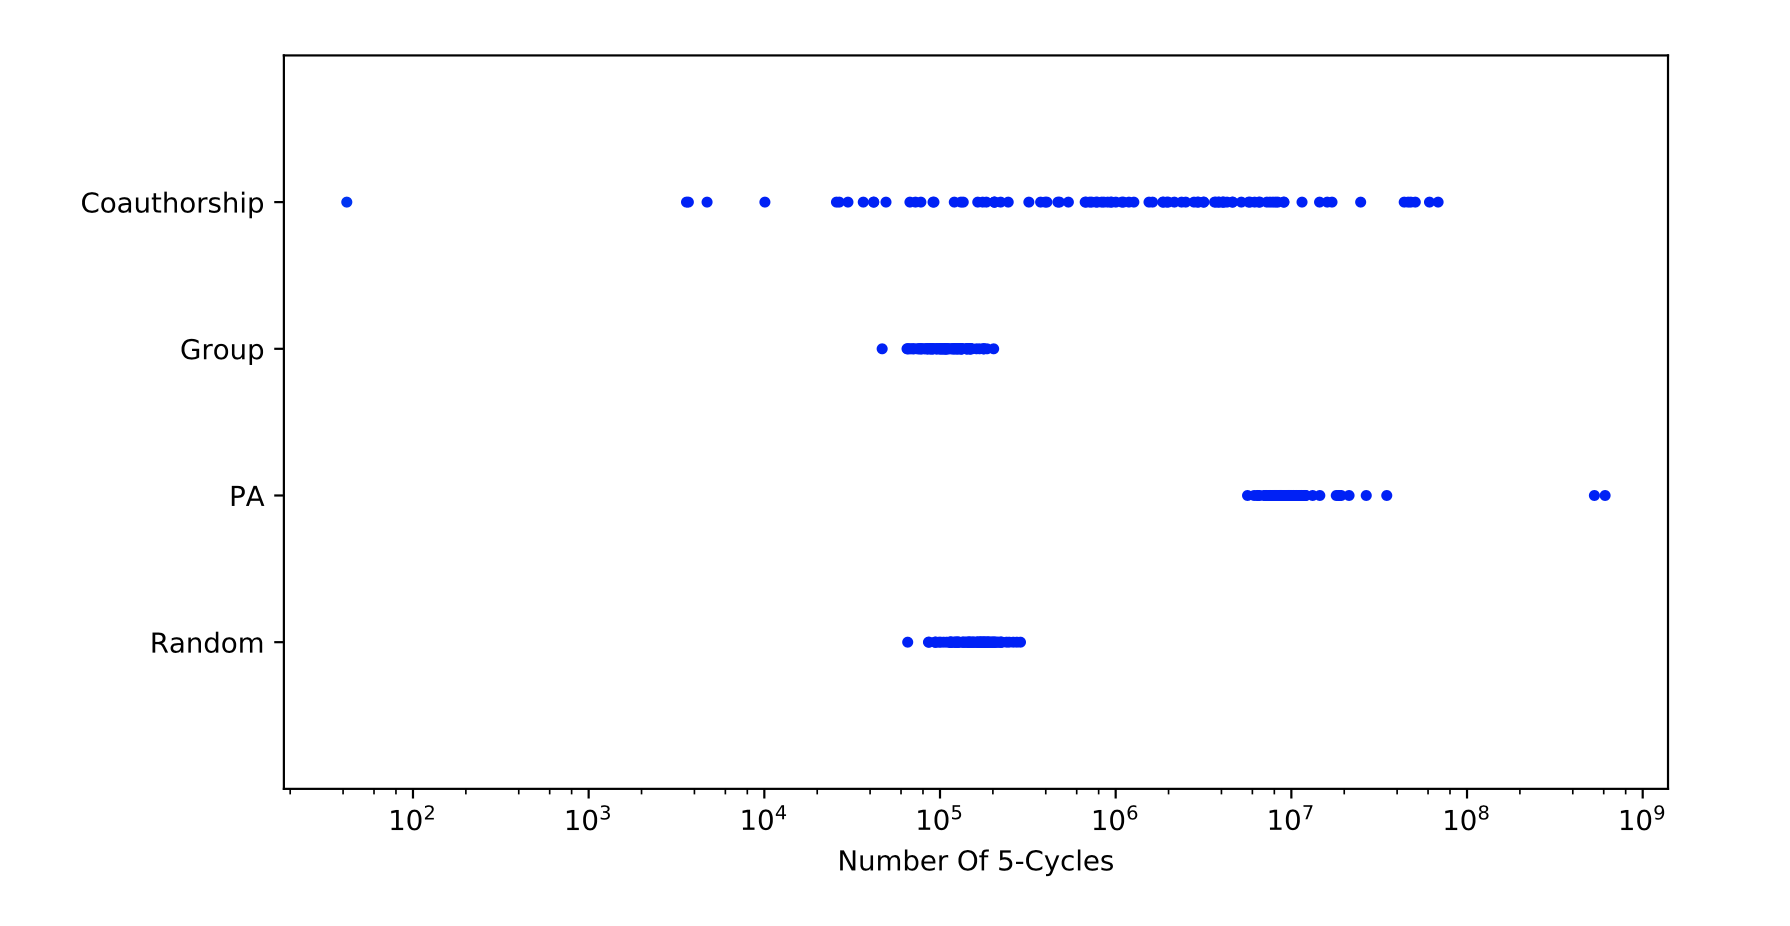
\includegraphics[width=0.75\textwidth]{pictures/5cycle.png}
\end{figure}

Figure 0.8 shows the number of 5-cycles that are present in each graph, this is very similar to the 4-cycle distribution, however there are obviously fewer due to the higher number of nodes required to make up a 5-cycle. The same parameters were used in each of the graphs and thus they show a very similar distribution for the same reasons as the 4-cycle distributions.

%%%%%%%%%%%%%%%%%%%%%%%%%%%%%%%%%%%%%%%%%%%%%%%%%%
\section*{Question Three}

Given a start and end vertex in a given graph find the search time, that being the average number of 'steps' or edges between two vertices in the given graph. For random, PA, and group graphs describe a search strategy, at each step using only local information which vertex to move to next. Explain why the strategy might be effective and implement and test it. Plot search time against the number of instances that achieve that time.

\subsection*{Random}

By their definition random graphs are random and due to this the search strategy will incorporate a certain degree of randomisation. The logic here is to move around the graph randomly until a node is reached that is adjacent to the end node. A random graph means that we cannot infer any details about the structure of the graph, meaning we cannot add any more specialisation to this method. \\

\begin{algorithm}[H]
 At start node\;
 \While{not at end node}{
  \eIf{end node in neighbours[current node]}{
   go to end node\;
   }{
   choose random unvisited neighbouring node\;
   got to this node\;
  }
 }
 \caption{Random Strategy}
\end{algorithm}

\begin{figure}[h]
\center
\caption{}
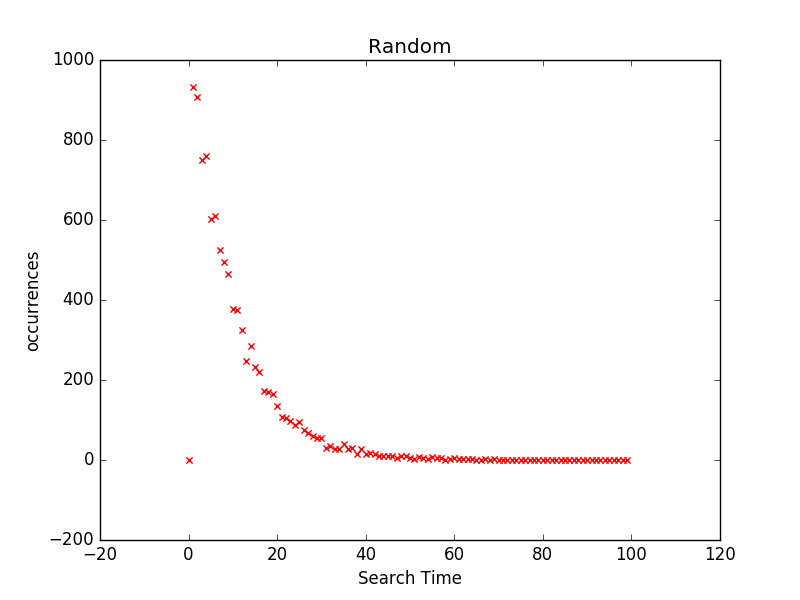
\includegraphics[width=0.75\textwidth]{pictures/randomSearch.png}
\end{figure}

For a random graph with 100 nodes and a connectivity probability of 0.05, as shown in figure 0.9, the most frequent search time is one. The average search time is 10.2. 

\subsection*{Preferential Attachment}

A PA graph is a fully connected graph that then has more nodes added to it. This means that the fully connected 'heart' of the graph is more likely to, firstly have more connections as well as having any 'extra nodes' connected to it. This will make up the core of the search strategy. The main focus of this search strategy is to get to the fully connected sub-graph which has a higher probability of being connected to the end node. If this fails then we visit nodes outside of this sub-graph and hope that they are connected to the end node. If we can avoid going to a node we have already been to then we will but if there is not other options then we will have to.\\

\begin{algorithm}[H]
 At start node\;
 \While{not at end node}{
  \eIf{end node in neighbours[current node]}{
   go to end node\;
   }{
   \Switch{unvisted nodes in complete subgraph}
   {choose one at random\;
   go to it\;}
   \Case{unvisited nodes outside complete subgraph}
   {choose one at random\;
   go to it\;}
   \Case{visited nodes in complete subgraph}
   {choose a random one\;
   go to it\;}
   \Other{choose a random neighbour\;
   go to it\;}
  }
 }
 \caption{PA Strategy}
\end{algorithm}

\begin{figure}[h]
\center
\caption{}
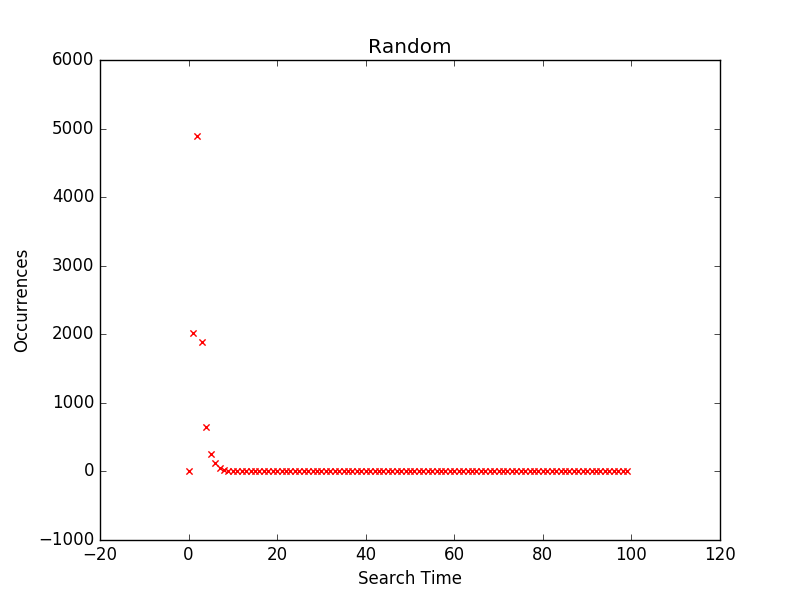
\includegraphics[width=0.75\textwidth]{pictures/paSearch.png}
\end{figure}

For a PA graph with 100 nodes and put degree of 15, the most frequent search time is two and the average search time is 2.27.

\subsection*{Group}

The group graph takes in four parameters to decide is structure, m, the number of groups in the graph, k, the size of each group, the graph has m * k nodes, p, the probability of two nodes in the same group have an edge between them, q, the probability of two nodes not in the same group have an edge between them.

We will take into consideration the predetermined structure of the graph in the search strategy. For this search algorithm the parameters that are used to create the graph are known and thus we can have a more specialised search algorithm as we can infer from the parameters an insight into the structure of the graph. For a high P value it can be infered that there is a high probability of intra-group edges, meaning that it would be optimal to aim for the group that the end node is in as there is a high probability it is connected to any other node in its group. For a high Q value it can be infered that there is a high probability that there are inter-group edges and low probability that there exist intra-group edges so aiming for the group of the end node will be of very little help, so this will be avoided. The final case is where P and Q have very similar values and therefore the structure of the graph is similar to that of a random graph, thus we re-use the random graph algorithm.\\

\begin{algorithm}[H]
 At start node\;
 \Switch{High p value}{

 \While{not at end node}
 {
 \eIf{end node in neighbours[current node]}
  {go to end node\;}
  {\eIf{any nodes in neighbours[current node] and in end group}{choose one at random\; go to it\;}{choose a random neighbour\; go to it\;}}
 }
 
 }
 \Case{High q value}{
 
 \While{not at end node}
 {
 \eIf{end node in neighbours[current node]}
  {go to end node\;}
  {\eIf{any nodes in neighbours[current node] but not in end group}{choose one at random\; go to it\;}{choose a random neighbour\; go to it\;}}
 }
 
 }
 \Other
{
  \While{not at end node}{
  \eIf{end node in neighbours[current node]}{
   go to end node\;
   }{
   choose random unvisited neighbouring node\;
   got to this node\;
  }
 }
 }
 \caption{Group Strategy}
\end{algorithm}

\begin{figure}[h]
\center
\caption{}
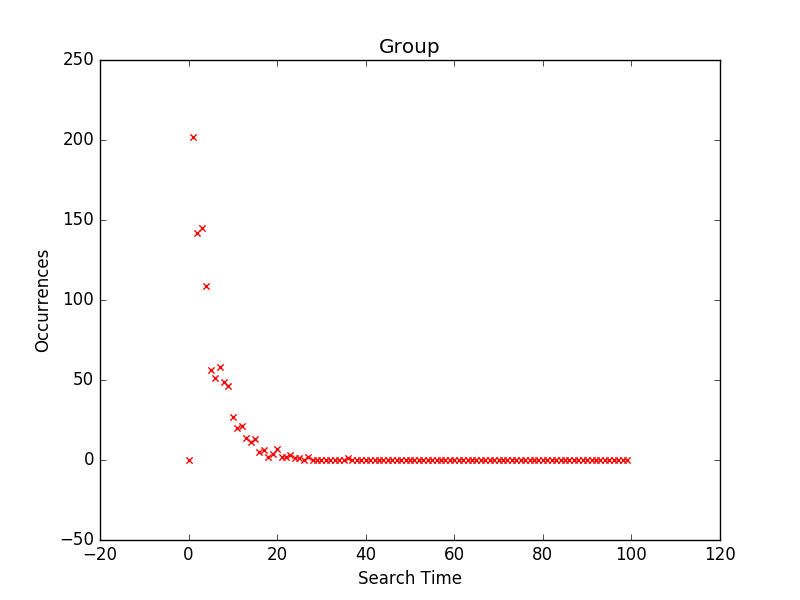
\includegraphics[width=0.75\textwidth]{pictures/groupSearch.png}
\end{figure}

For a group graph with m = 40, k = 40, p = 0.4, and q = 0.1, as shown in figure 0.11 the most frequent search time was one with the average search time being 5.2.


%%%%%%%%%%%%%%%%%%%%%%%%%%%%%%%%%%%%%%%%%%%%%%%%%%
%%% End document
\end{document}